\chapter{Análise Estatística do Desempenho do Sistema de Recomendação}\label{ape:analise-estatistica-do-uso}

\section{Links Acessados por Aluno}

\begin{figure}[htb]
  \caption{\label{fig:uso-sr-boxplot}Boxplot dos links acessados por aluno}
  \begin{center}
      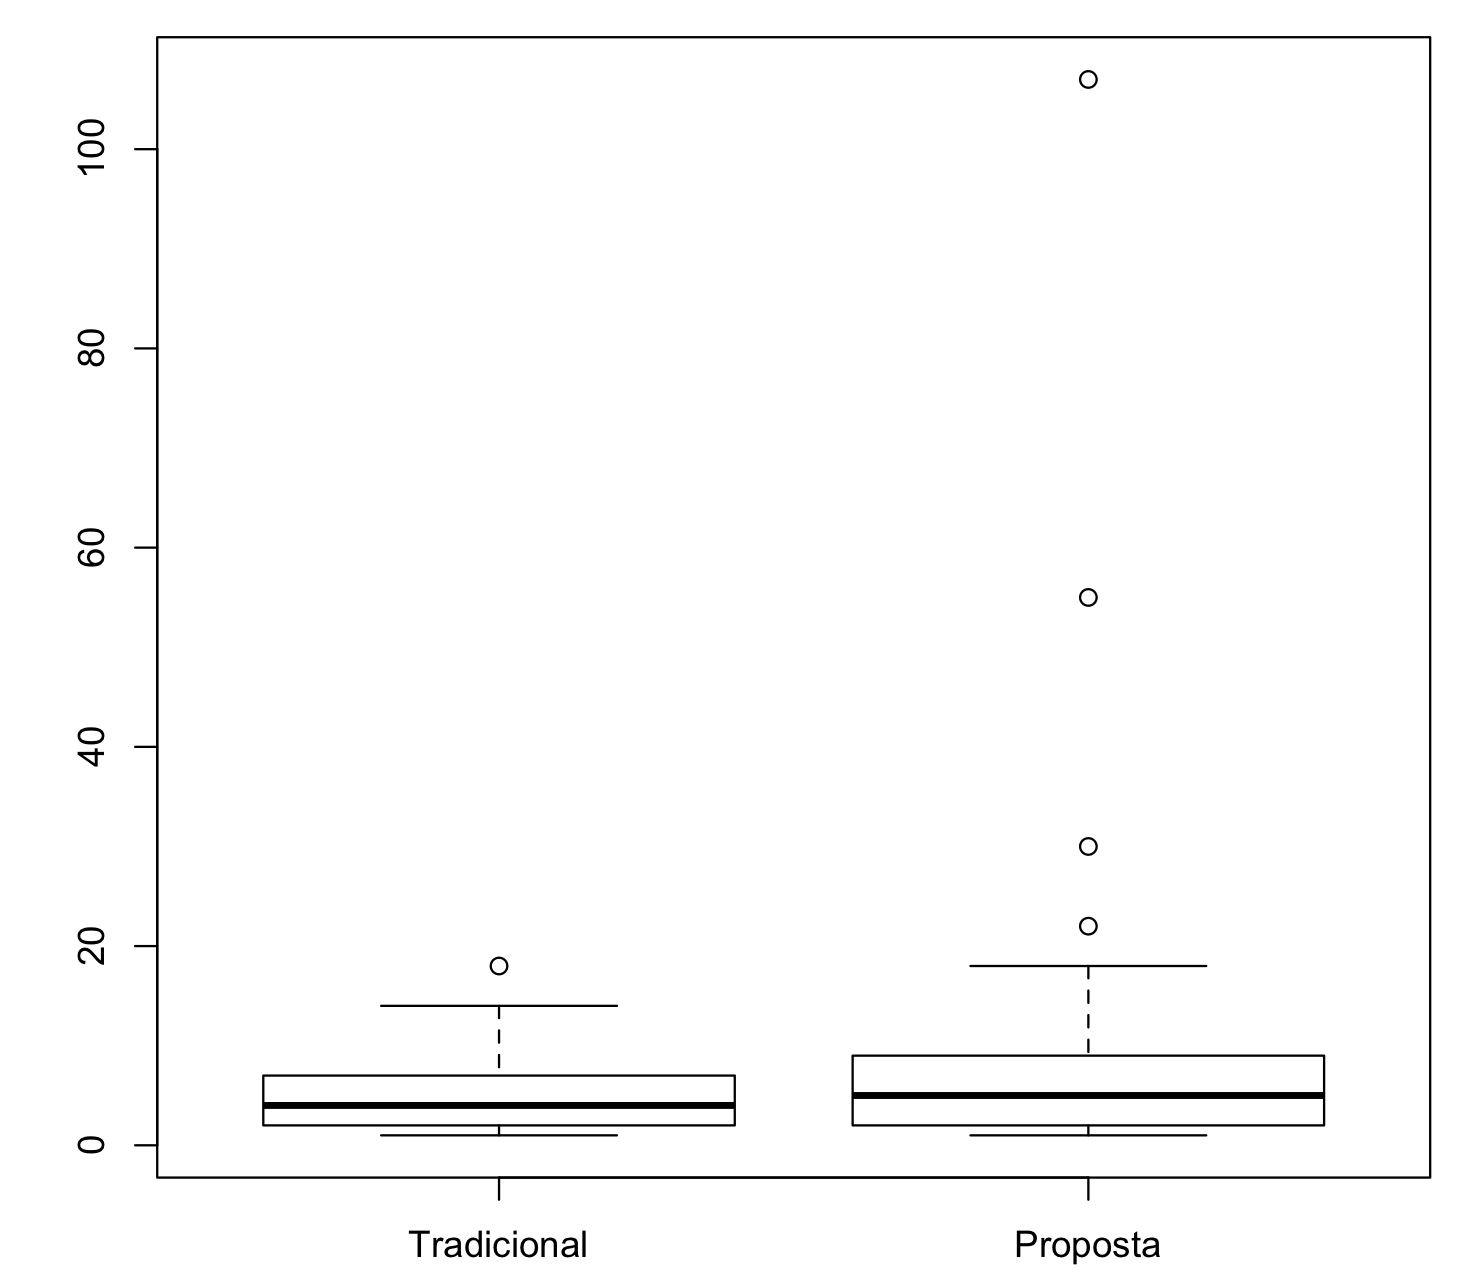
\includegraphics[scale=0.4]{./Figuras/uso-sr-boxplot.png}
  \end{center}
  \legend{Fonte: O autor.}
\end{figure}

\noindent
Total de alunos comparados: 85

\begin{table}[h]
\begin{tabular}{p{.50\textwidth}p{.50\textwidth}}
  \textbf{Tradicional} & \textbf{Proposta} \\
  Min = 1.000 & Min = 1.00 \\
  1\textsuperscript{o} Quad = 2.000 & 1\textsuperscript{o} Quad = 2.00 \\
  Mediana = 4.000 & Mediana = 5.00 \\
  Média = 4.935 & Média =  10.15 \\
  3\textsuperscript{o} Quad = 6.500 & 3\textsuperscript{o} Quad = 9.00 \\
  Max = 18.000 & Max = 107.00 \\
\end{tabular}
\end{table}

Shapiro-Wilk normality test

\noindent
data:  data[["quantidade"]]\\
W = 0.42461, p-value < 2.2e-16

\noindent
\textbf{Resultado: Aceita a hipótese alternativa - Distribuição não normal}

Wilcoxon rank sum test with continuity correction

\noindent
data:  data[["quantidade"]] by data[["algoritmo\_recomendacao"]]\\
W = 820, p-value = 0.4957\\
alternative hypothesis: true location shift is not equal to 0

\noindent
\textbf{Resultado: Aceita a hipótese nula - Sem diferença significativa}

\newpage
\section{Links Avaliados Positivamente por Aluno}

\begin{figure}[htb]
  \caption{\label{fig:avaliados-positivamente-boxplot}Boxplot dos links avaliados positivamente por aluno}
  \begin{center}
      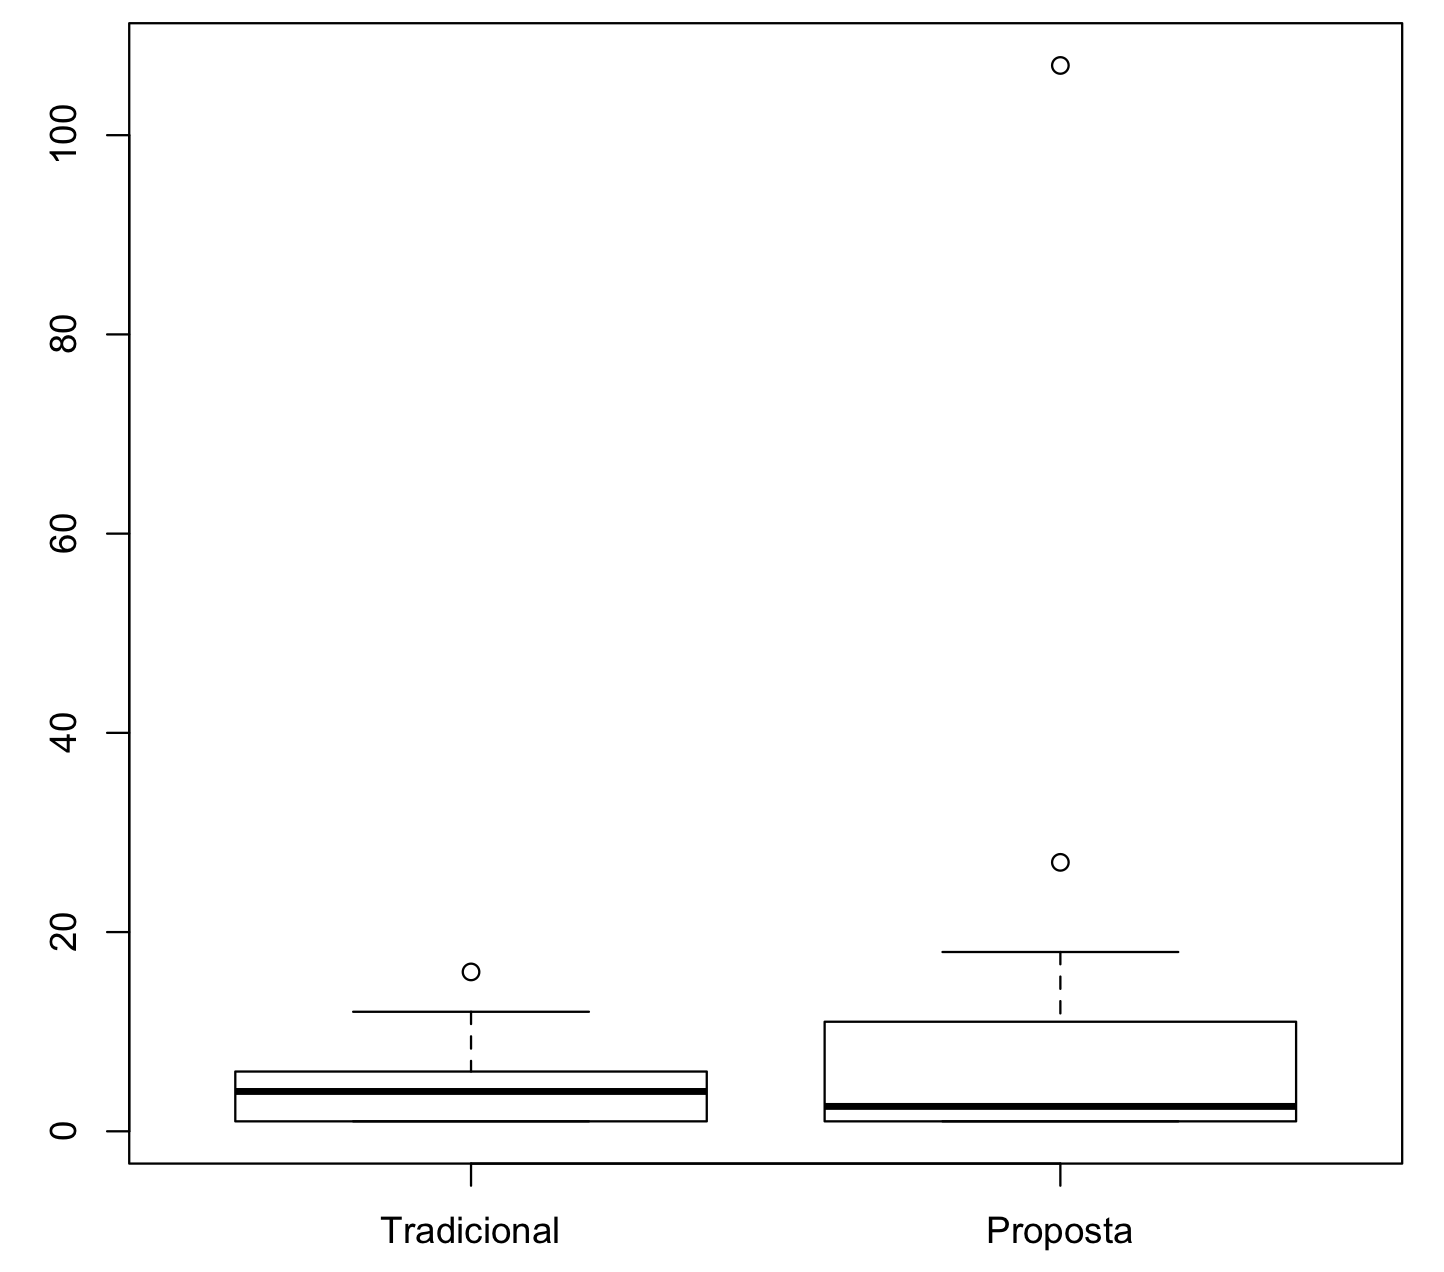
\includegraphics[scale=0.4]{./Figuras/avaliados-positivamente-boxplot.png}
  \end{center}
  \legend{Fonte: O autor.}
\end{figure}

\noindent
Total de alunos comparados: 52

\begin{table}[h]
\begin{tabular}{p{.50\textwidth}p{0.5\textwidth}}
\textbf{Tradicional} & \textbf{Proposta}\\
Min =  1.0 & Min =   1.00\\
1\textsuperscript{o} Quad = 1.0 & 1\textsuperscript{o} Quad = 1.00\\
Mediana =  4.0 & Mediana =   2.50\\
Média =  4.7 & Média =  10.64\\
3\textsuperscript{o} Quad = 6.0 & 3\textsuperscript{o} Quad = 9.75\\
Max = 16.0 & Max = 107.00\\
\end{tabular}
\end{table}

  Shapiro-Wilk normality test

\noindent
data:  data[["quantidade"]]\\
W = 0.37836, p-value = 1.654e-13

\noindent
\textbf{Resultado: Aceita a hipótese alternativa - Distribuição não normal}

Wilcoxon rank sum test with continuity correction

\noindent
data:  data[["quantidade"]] by data[["algoritmo\_recomendacao"]]\\
W = 318, p-value = 0.8275\\
alternative hypothesis: true location shift is not equal to 0

\noindent
\textbf{Resultado: Aceita a hipótese nula - Sem diferença significativa}

\newpage
\section{Links avaliados negativamente por aluno que acessou pelo menos uma recomendação}

\begin{figure}[htb]
  \caption{\label{fig:uso-sr-boxplot}Boxplot dos links acessados por aluno}
  \begin{center}
      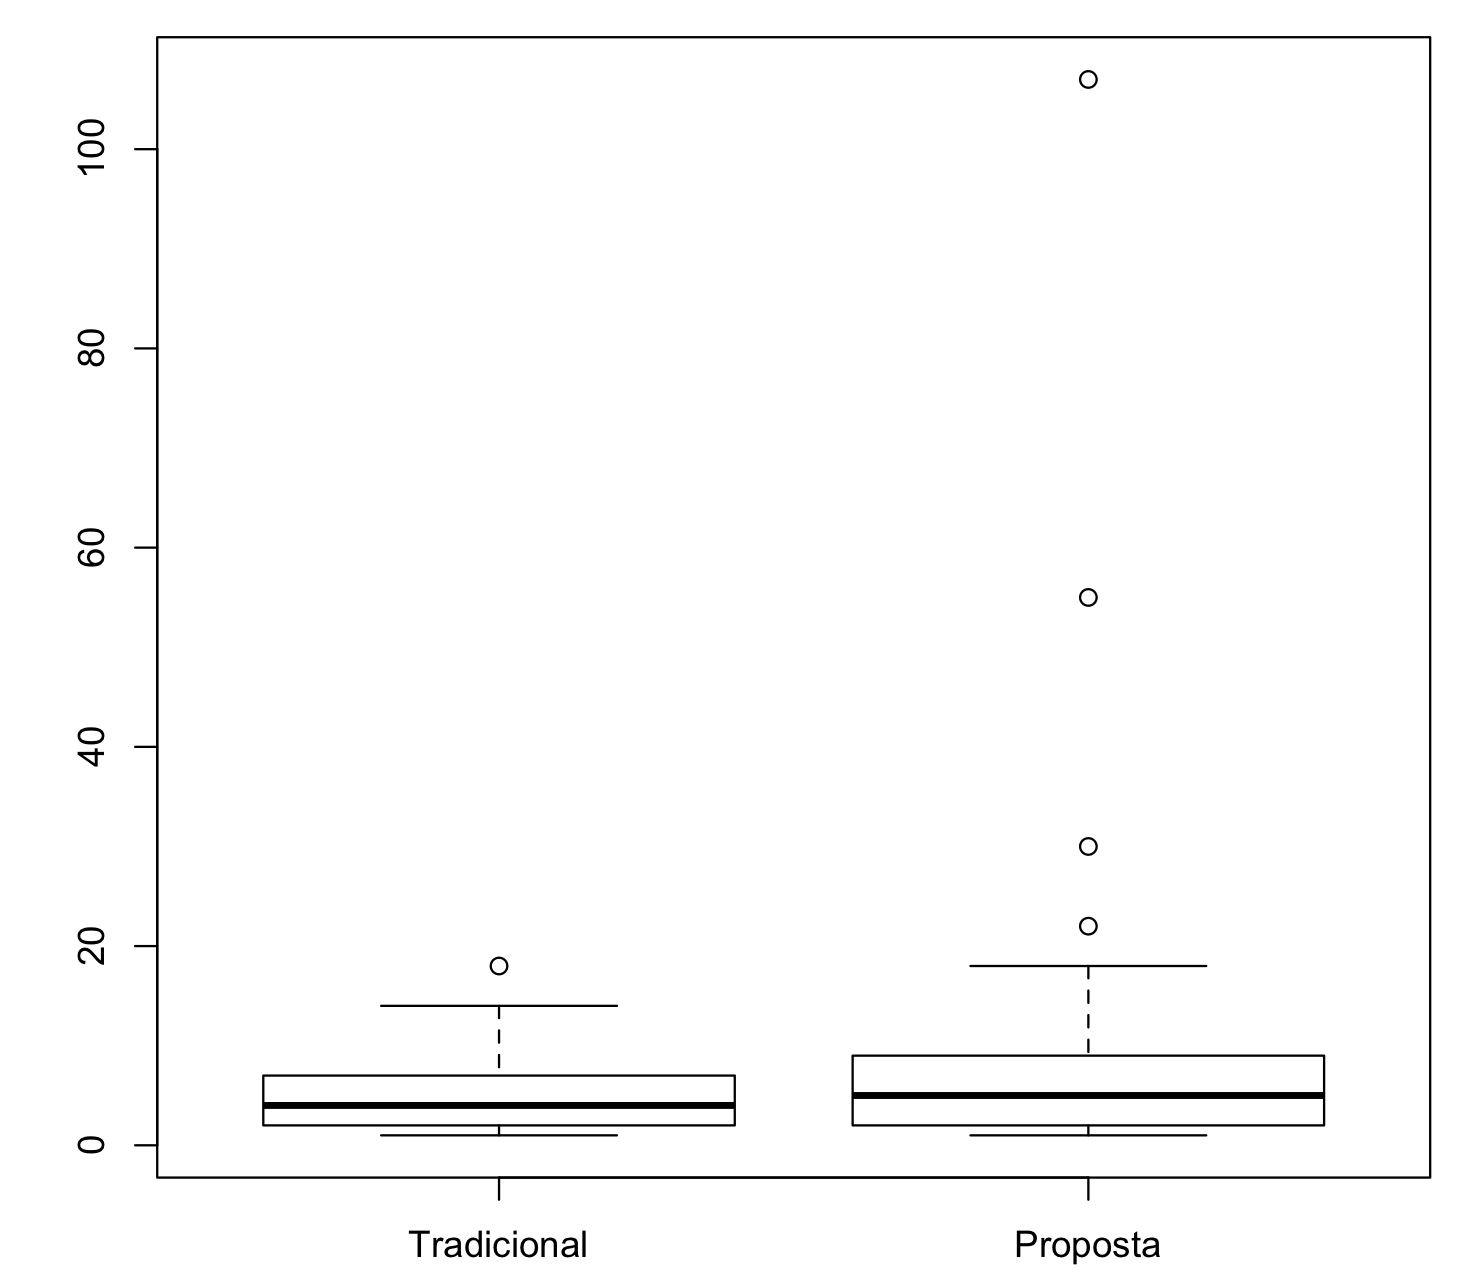
\includegraphics[scale=0.4]{./Figuras/uso-sr-boxplot.png}
  \end{center}
  \legend{Fonte: O autor.}
\end{figure}

\noindent
Total de alunos comparados: 7

\begin{table}[h]
\begin{tabular}{p{.50\textwidth}p{0.5\textwidth}}
\textbf{Tradicional} & \textbf{Proposta}\\
Min = 1 & Min = 1.0\\
1\textsuperscript{o} Quad = 1 & 1\textsuperscript{o} Quad = 1.5\\
Mediana = 1 & Mediana = 2.0\\
Média = 1 & Média = 2.0\\
3\textsuperscript{o} Quad = 1 & 3\textsuperscript{o} Quad = 2.5\\
Max = 1 & Max = 3.0\\
\end{tabular}
\end{table}

  Shapiro-Wilk normality test

\noindent
data:  data[["quantidade"]]\\
W = 0.45297, p-value = 4.136e-06

\noindent
\textbf{Resultado: Aceita a hipótese alternativa - Distribuição não normal}

Wilcoxon rank sum test with continuity correction

\noindent
data:  data[["quantidade"]] by data[["algoritmo\_recomendacao"]]\\
W = 2.5, p-value = 0.2059\\
alternative hypothesis: true location shift is not equal to 0

\noindent
\textbf{Resultado: Aceita a hipótese nula - Sem diferença significativa}

\newpage
\section{Precisão dos algoritmos de recomendação por aluno}

\begin{figure}[htb]
  \caption{\label{fig:precisao-boxplot}Boxplot da precisão dos algoritmos de recomendação por aluno}
  \begin{center}
      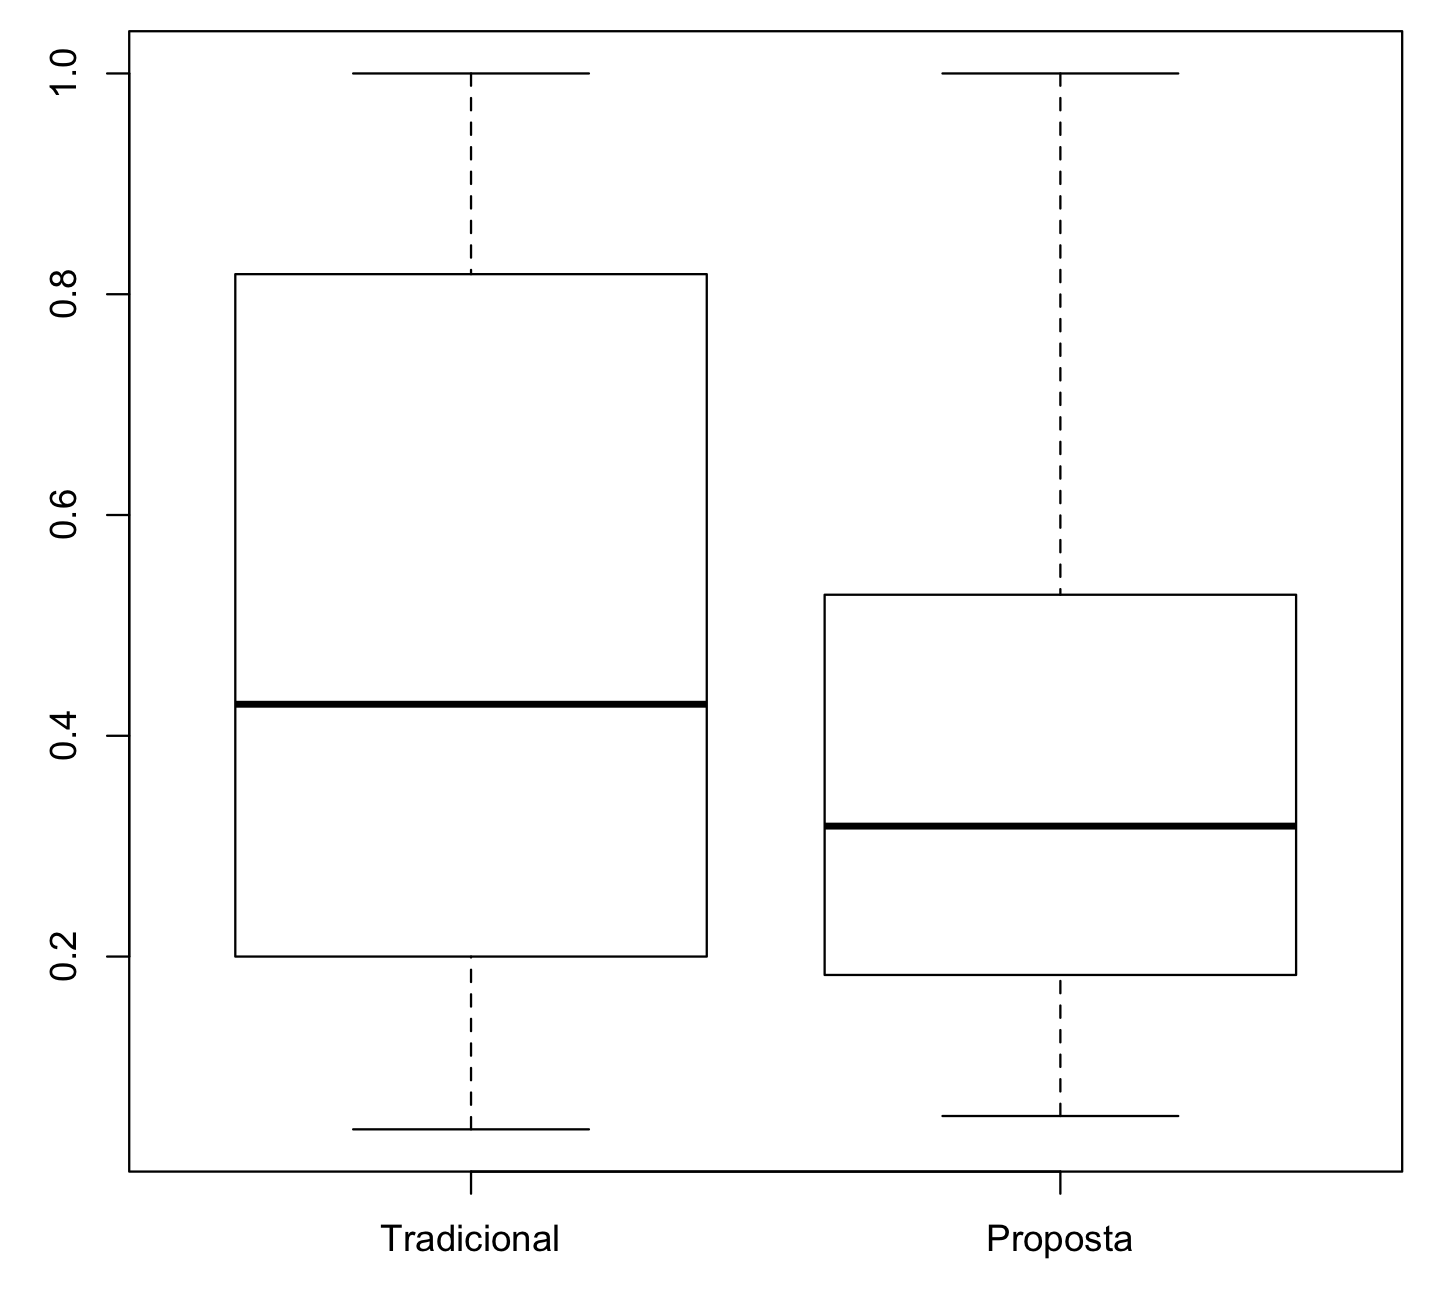
\includegraphics[scale=0.4]{./Figuras/precisao-boxplot.png}
  \end{center}
  \legend{Fonte: O autor.}
\end{figure}

\noindent
Total de alunos comparados: 85

\begin{table}[h]
\begin{tabular}{p{.50\textwidth}p{0.5\textwidth}}
\textbf{Tradicional} & \textbf{Proposta}\\
Min = 0.04348 & Min = 0.05556\\
1\textsuperscript{o} Quad = 0.20000 & 1\textsuperscript{o} Quad = 0.18333\\
Mediana = 0.42857 & Mediana = 0.31818\\
Média = 0.49679 & Média = 0.39859\\
3\textsuperscript{o} Quad = 0.81364 & 3\textsuperscript{o} Quad = 0.52778\\
Max = 1.00000 & Max = 1.00000\\
\end{tabular}
\end{table}

  Shapiro-Wilk normality test

\noindent
data:  data[["precisao"]]\\
W = 0.89495, p-value = 4.234e-06

\noindent
\textbf{Resultado: Aceita a hipótese alternativa - Distribuição não normal}

Wilcoxon rank sum test with continuity correction

\noindent
data:  data[["precisao"]] by data[["algoritmo\_recomendacao"]]\\
W = 1025, p-value = 0.2603\\
alternative hypothesis: true location shift is not equal to 0

\noindent
\textbf{Resultado: Aceita a hipótese nula - Sem diferença significativa}

\newpage
\section{Cobertura dos algoritmos de recomendação por aluno}

\begin{figure}[htb]
  \caption{\label{fig:coverage-boxplot}Boxplot da cobertura dos algoritmos de recomendação por aluno}
  \begin{center}
      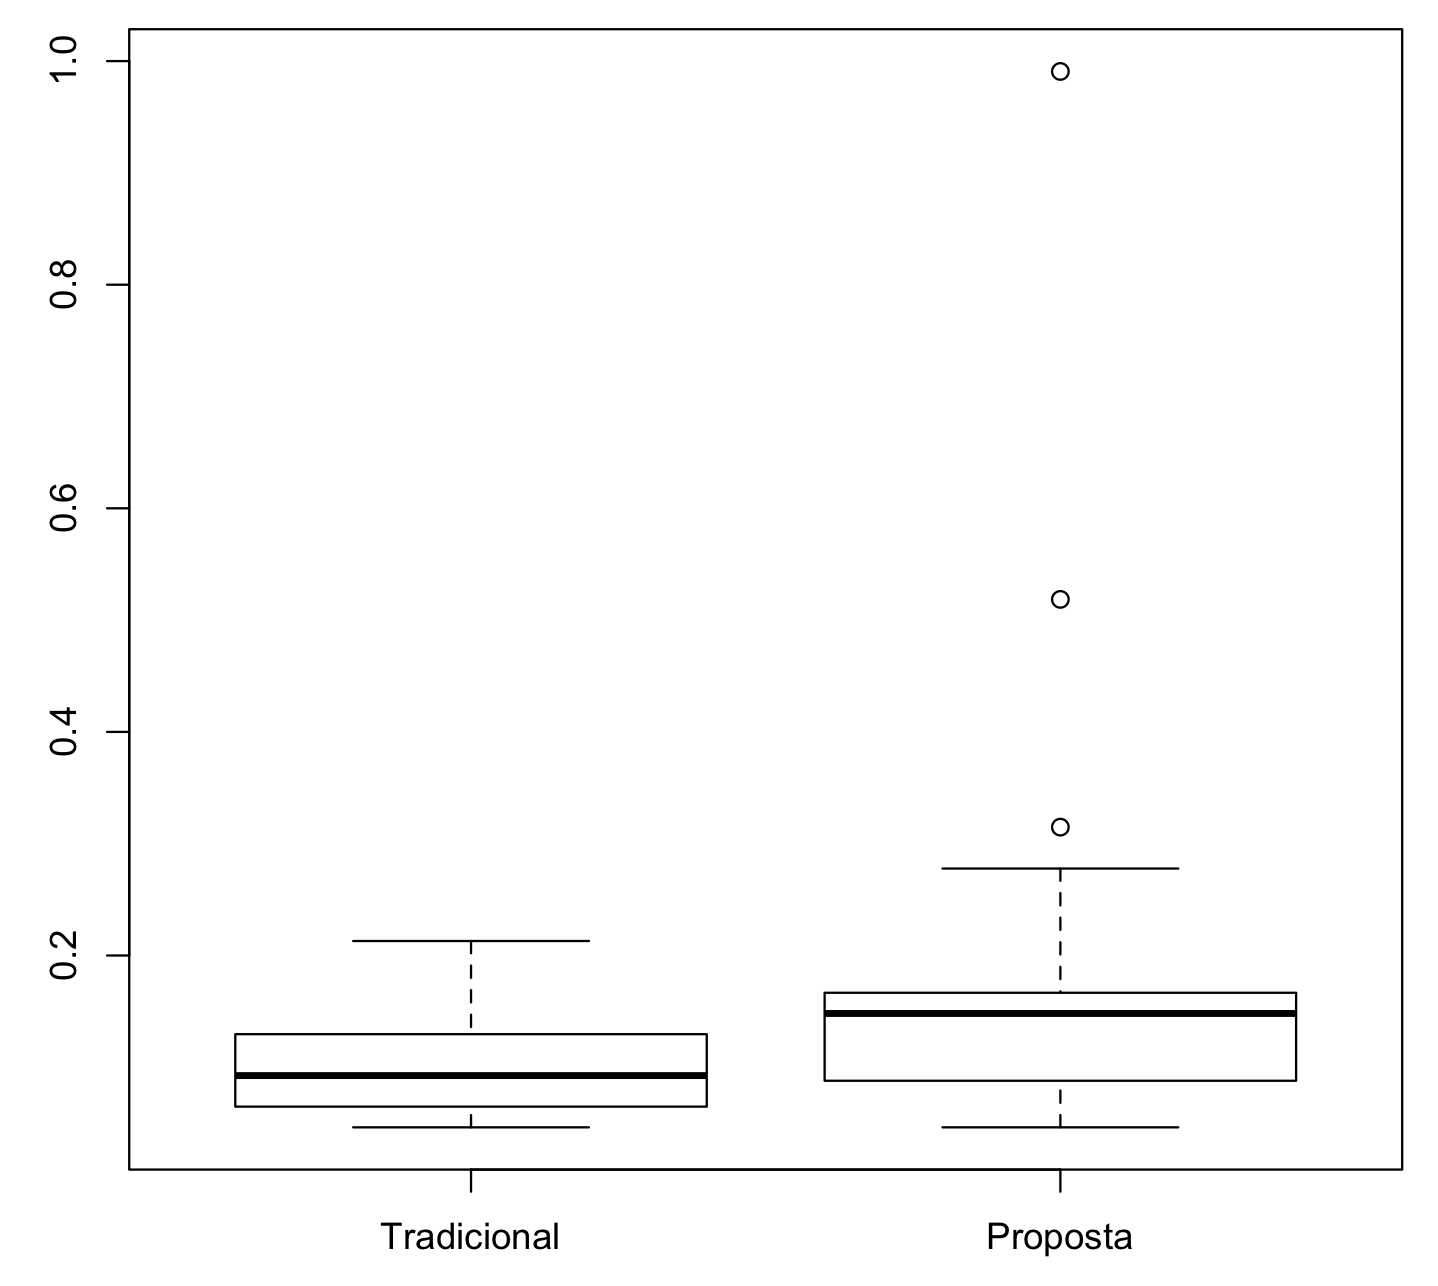
\includegraphics[scale=0.4]{./Figuras/coverage-boxplot.png}
  \end{center}
  \legend{Fonte: O autor.}
\end{figure}

\noindent
Total de alunos comparados: 85

\begin{table}[h]
\begin{tabular}{p{.50\textwidth}p{0.5\textwidth}}
\textbf{Tradicional} & \textbf{Proposta}\\
Min = 0.04630 & Min = 0.04630\\
1\textsuperscript{o} Quad = 0.06481 & 1\textsuperscript{o} Quad = 0.08796\\
Mediana = 0.09259 & Mediana = 0.14815\\
Média = 0.10064 & Média = 0.17450\\
3\textsuperscript{o} Quad = 0.12963 & 3\textsuperscript{o} Quad = 0.16667\\
Max = 0.21296 & Max = 0.99074\\
\end{tabular}
\end{table}

    Shapiro-Wilk normality test

\noindent
data:  data[["coverage"]]\\
W = 0.55934, p-value = 1.421e-14

\noindent
\textbf{Resultado: Aceita a hipótese alternativa - Distribuição não normal}

  Wilcoxon rank sum test with continuity correction

\noindent
data:  data[["coverage"]] by data[["algoritmo\_recomendacao"]]\\
W = 525.5, p-value = 0.001031\\
alternative hypothesis: true location shift is not equal to 0

\noindent
\textbf{Resultado: Aceita a hipótese alternativa - Com diferença significativa}

\newpage
\section{F-measure do algoritmo de recomendação por aluno}

\begin{figure}[htb]
  \caption{\label{fig:media-harmonica-boxplot}Boxplot do F-measure dos dois algoritmos}
  \begin{center}
      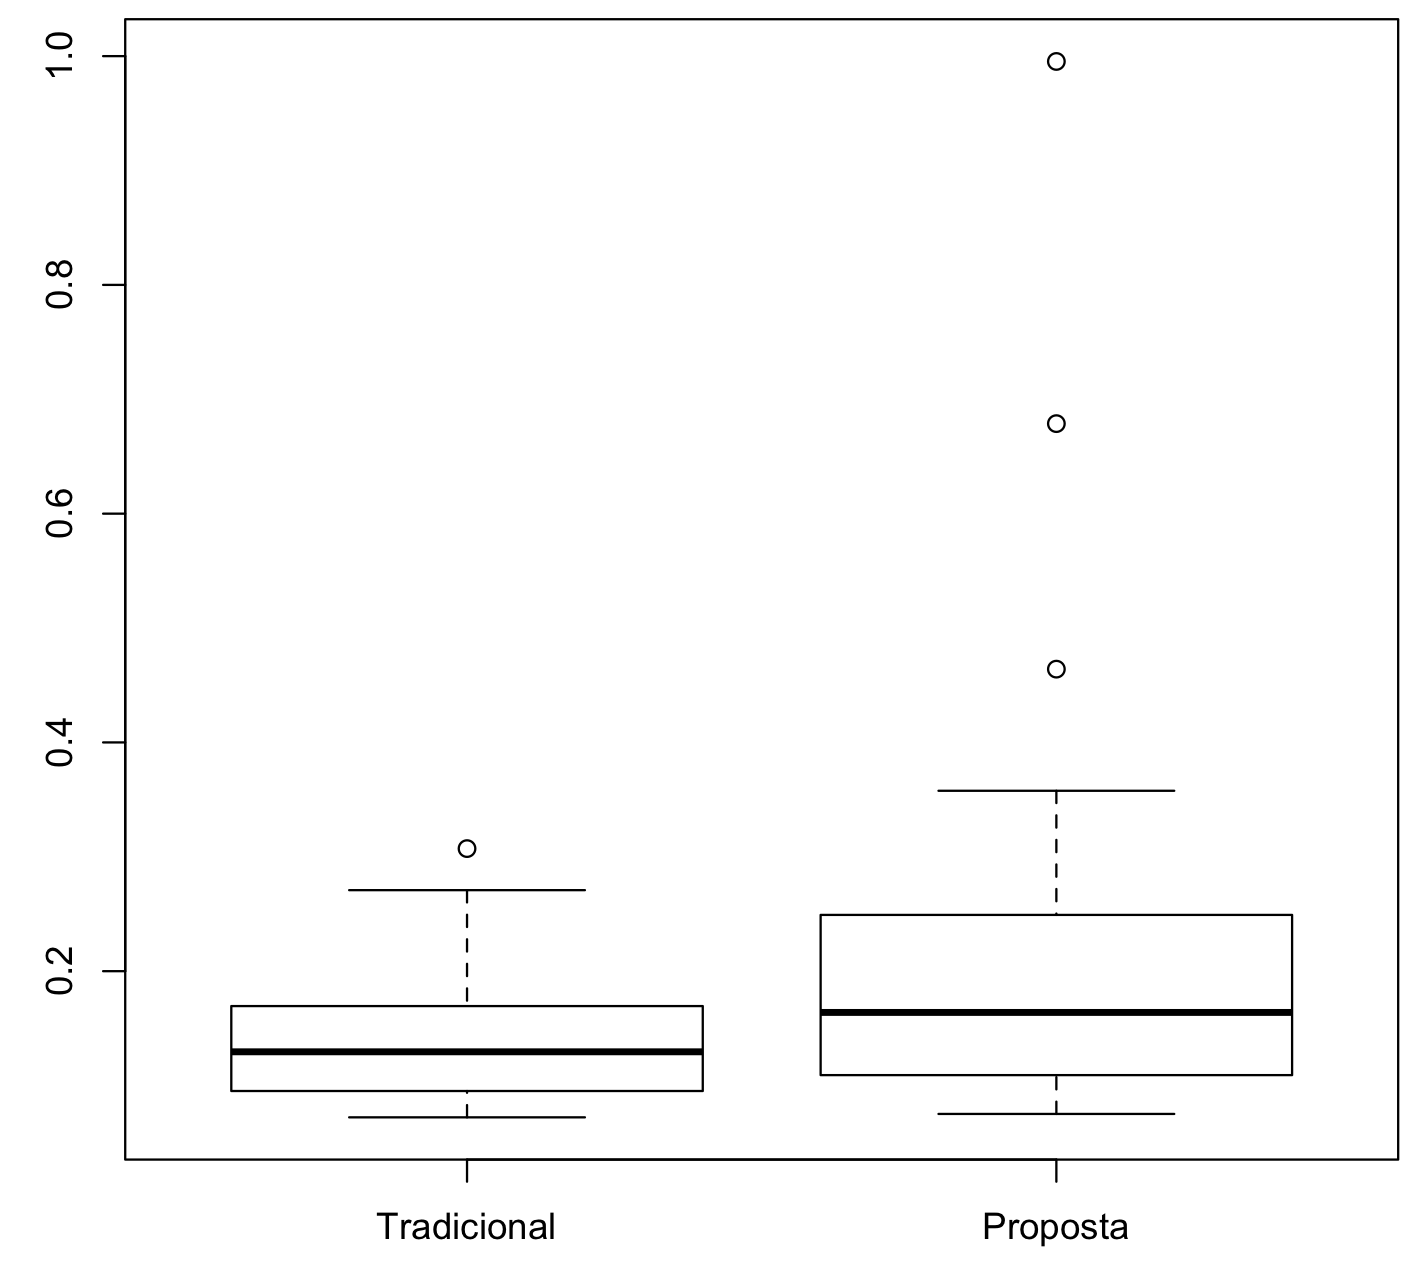
\includegraphics[scale=0.4]{./Figuras/media-harmonica-boxplot.png}
  \end{center}
  \legend{Fonte: O autor.}
\end{figure}

\noindent
Total de alunos comparados: 85

\begin{table}[h]
\begin{tabular}{p{.50\textwidth}p{0.5\textwidth}}
\textbf{Tradicional} & \textbf{Proposta}\\
Min = 0.07221 & Min = 0.07519\\
1\textsuperscript{o} Quad = 0.09545 & 1\textsuperscript{o} Quad = 0.10913\\
Mediana = 0.12952 & Mediana = 0.16393\\
Média = 0.13852 & Média = 0.21719\\
3\textsuperscript{o} Quad = 0.16618 & 3\textsuperscript{o} Quad = 0.24919\\
Max = 0.30717 & Max = 0.99535\\
\end{tabular}
\end{table}

Shapiro-Wilk normality test

\noindent
data:  data[["media\_harmonica"]]\\
W = 0.63292, p-value = 2.931e-13

\noindent
\textbf{Resultado: Aceita a hipótese alternativa - Distribuição não normal}

Wilcoxon rank sum test with continuity correction

\noindent
data:  data[["media\_harmonica"]] by data[["algoritmo\_recomendacao"]]\\
W = 634.5, p-value = 0.02082\\
alternative hypothesis: true location shift is not equal to 0

\noindent
\textbf{Resultado: Aceita a hipótese alternativa - Com diferença significativa}
